\section{Durchführung und Auswertung}

\subsection{Kernradienbestimmung}

Mithilfe der Am-Be-Neutronenquelle sollen im eigentlichen Versuchsteil nun die Kernradien verschiedener Absorbermaterialien bestimmt werden. 
Dafür benötigt man den totalen Wirkungsquerschnitt der Reaktion der Neutronen im Absorber. Diesen kann man über die verschiedenen Zählraten der eingesetzten Absorber wie folgt bestimmen:

\begin{align}
Z=Z_=\cdot e^{-\mu d}
\end{align}

Dabei entspricht Z der Zählrate mit Absorber, $Z_0$ der Zählrate ohne Absorber, d der Dicke des Absorber und $\mu$ dem sogenannten Schwächungskoeffzienten, welcher wie folgt mit dem totalen Wirkungsquerschnitt $\sigma_{tot} = 2\pi R^2$ und der Zahl der Kerne pro $cm^3$ N zusammenhängt:

\begin{align}
\mu=\sigma_{tot}\cdot N 
\end{align}

Über die verschiedenen Zählraten können so $\mu$, $\sigma_{tot}$ und damit R bestimmt werden. Die bestimmten Werte können anschließend zur Bestimmung der Radiuskonstante $r_0$ verwendet werden, da folgende Beziehung gilt:

\begin{align}
R=r_0 \cdot A^{1/3}
\end{align}

Da das Neutron weiterhin nur bis auf eine reduzierte De-Broglie-Wellenlänge lokalisiert werden kann, ergibt sich die reduzierte De-Broglie-Wellenlänge $\lambda_{dB}$ als Offset der gerade genannten Beziehung.

Für die Messung werden die verschiedenen Absorber in die in Abschnitt 3 bestimmte Position gebracht und die entsprechenden Spektren mit einer Messdauer von 1920s vermessen. Weiterhin werden nur Neutronen mit einer Energie von über 7MeV als "richtige" Neutronen angenommen, da der oben angenommene Wirkungsquerschnitt nur in diesem Energiebereich gültig ist. Dafür muss bei der Bestimmung der Zählrate der richtige Bereich des 2D-Histogramms ausgewählt werden, wobei hier nur 128 Kanäle vorhanden sind. Über die oben schon dargestellte Energierelation zwischen Neutronen und Elektronen, kann eine minimale Elektron-Energie von 3MeV identifiziert werden. Im schon kalibrierten Energie-Diagramm mit 2014 Kanälen entspricht dies allen Ereignissen ab Kanal 562. Umgerechnet auf 128 Kanäle müssen wir also alle Neutronen-Ereignisse ab Kanal 71 zählen, um auf die korrekte Zählrate zu kommen. Die bei den verschiedenen Absorbern aufgenommenen Zählraten gemeinsam mit den Atommassen und Dichten der Absorbermaterialien finden sich in den Tabellen \ref{werte} und \ref{werte2}. 

\begin{table}[h]
	\caption{Neutronen-Zählraten mit verschiedenen Absorbermaterialien}
	\begin{tabular}{|c|c|c|c|c|c|}
	\hline
	 Absorber & Zählrate & $\mu$ & $\sigma$ & R & $A^\frac{1}{3}$ \\ \hline
	  ohne & 23713 &  &  &  & &  &   \\ \hline
	   Cadmium & 10785  & 0,157 & $3,4\cdot 10^{-24}$ & $7,36 \cdot 10^{-13}$ & 4,83\\ \hline
	    Aluminium & 13459 & 0,113 & $3,4\cdot 10^{-24}$ & $5,48 \cdot 10^{-13}$  & 3 \\ \hline
	     Blei & 10714  & 0,159 & $3,4\cdot 10^{-24}$ & $8,77 \cdot 10^{-13}$  & 5,92 \\ \hline
	      Eisen & 7434  & 0,232 & $3,4\cdot 10^{-24}$ & $6,59 \cdot 10^{-13}$  & 3,82 \\ \hline
	       Kupfer & 6990 & 0,244 & $3,4\cdot 10^{-24}$ & $6,78 \cdot 10^{-13}$  & 3,99\\ \hline
	\end{tabular}
\label{werte}
\end{table}

\begin{table}[h]
	\caption{Daten Absorbermaterialien}
	\begin{tabular}{|c|c|c|}
	\hline
	 Absorber & Atommasse in u & Dichte in g/$cm^3$ & Teilchen / $cm^3$ \\ \hline
	   Cadmium & 112,4  & 8,65 & $4,63 \cdot 10^{22}$ \\ \hline
	    Aluminium & 27 & 2,69 & $5,99 \cdot 10^{22}$ \\ \hline
	     Blei & 207  & 11,3 & $3,28 \cdot 10^{22}$  \\ \hline
	      Eisen & 55,8  & 7,87 & $8,49 \cdot 10^{22}$ \\ \hline
	       Kupfer & 63,5 & 8,92 & $8,45 \cdot 10^{22}$ \\ \hline
	\end{tabular}
\label{werte2}
\end{table}

Die bestimmten Werte für R können gegenüber der dritten Wurzel der Massenzahl aufgetragen und aus der Steigung die Radiuskonstante $r_0$ und aus dem y-Achsenabschnitt die De-Broglie-Wellenlänge bestimmt werden. In Abbildung \ref{kernradien} findet sich dieser Plot. Als fehlerbehaftete Größen wurden die Dicke der Absorber und die Zählraten angenommen, wobei der Fehler der Absorberdicke auf $\Delta d = 1mm$ geschätzt wurde, während die Zählraten als normalverteilte Größen und damit mit einem Fehler von $\sqrt{Z}$ behaftet angenommen wurden. Der Fehler für R ergibt sich dann zu:
\begin{align} 
\Delta R = R \left(\frac{\Delta d}{2d}\right) + \frac{\Delta Z_0}{2Z_0\log\frac{Z_0}{Z}}+\frac{\Delta Z}{2Z\log\frac{Z_0}{Z}}
\end{align}

\begin{figure}[htbp]  
     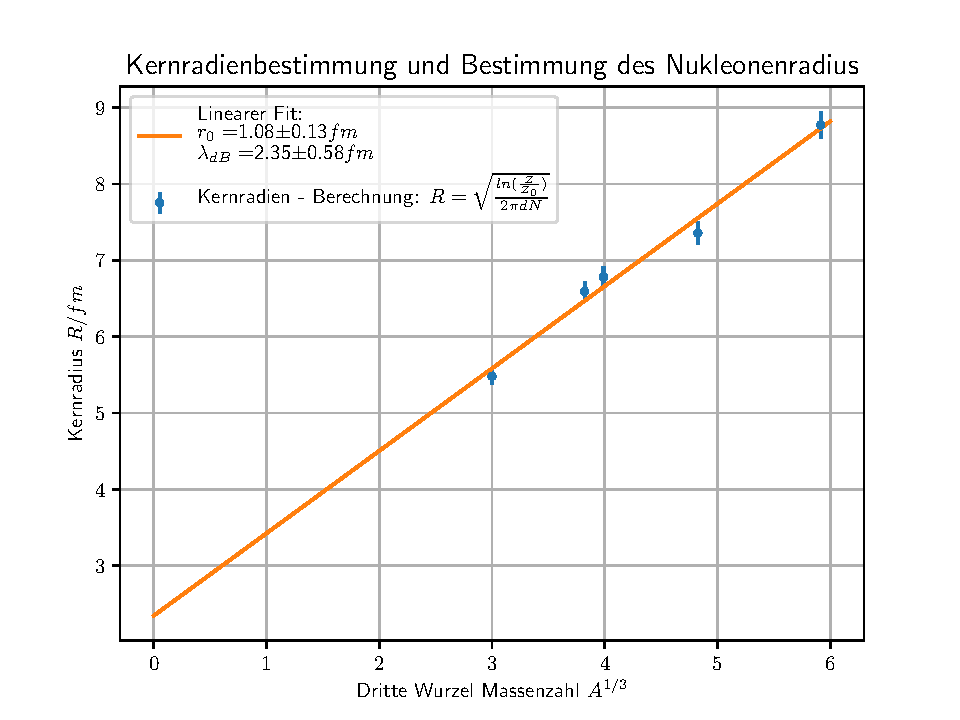
\includegraphics{kernradien.pdf}
  \caption{Kernradien über der dritten Wurzel der Massenzahl}
  \label{kernradien}
\end{figure}

Als Ergebnis finden wir so eine Radiuskonstante von $r_0=1,08 \pm 0,13 fm$. Der Literaturwert beträgt hier $\approx 1,2 fm$, unsere Messung ergibt also innerhalb der Fehlergrenzen einen absolut plausiblen und guten Wert. Unser Wert für die De-Broglie-Wellenlänge beträgt für die Neutronen $\lambda_{dB}=2,35 \pm 0,58 fm$. Über die relativistische Energie-Impuls-Beziehung und die Definition der De-Broglie-Wellenlänge lässt sich daraus eine Neutronenenergie von 526 MeV ableiten. Dieser Wert erscheint jedoch sehr unrealistisch, da die typischen Neutronenenergien der verwendeten Quelle im 1-10MeV - Bereich liegen. Als mögliche Fehlerquellen sind hier auf jeden Fall die einfache Abschätzung des Wirkungsquerschnitts und die geometrischen Fehler der Absorber zu nennen.

\subsection{Time of Flight - Messung}

Für die Time-of-Flight-Messung wird aus den Daten der Messung der Kernradienbestimmung ohne Absorber die Lage der Peaks bestimmt. Die Abstände der beiden Detektoren zur Quelle betragen dabei einmal 50cm und einmal 3,15 cm. Im ToF-Spektrum treten dabei insgesamt 4 Peaks auf, welche aus den verschiedenen Kombinationen der Ansprechmöglichkeiten der beiden Detektoren resultieren. So kann ein bei der Kernreaktion entstehendes Neutron entweder im ersten oder im zweiten Detektor registriert werden, während der jeweils andere eines der entstehenden Photonen registrieren kann. Aus den unterschiedlichen Flugzeiten der Neutronen entstehen so die verschiedenen Peaks.

Die energiereichsten Neutronen sind im Spektrum durch den Peak mit der geringsten Zeitdifferenz zu finden. Über die Kanallage bei Kanal 493 und der geometrischen Abmessung des Aufbaus ergibt sich mit der vorausgegangenen Eichung eine kinetische Energie von 3,29 MeV für die Neutronen. Über das im Theorieteil gezeigte Zerfallsschema, wäre eigentlich eine Maximalenergie von 4,4 MeV zu erwarten gewesen, da die zu 50\% entstehende Zwischenstufe noch genau diese Anregungsenergie aufweist. Im Rahmen der vorliegenden Fehlerquellen (keine punktförmige Quelle, ungenaue Peakbestimmung, fehlerhafte Elektronik) ergibt unsere Messung jedoch eine gute Größenordnung. Die Neutronen besitzen mit dieser Energie ungefähr 10\% der Lichtgeschwindigkeit, sodass auch relativistische Effekte durchaus eine Begründung für die Abweichung darstellen. 
